% Author: Joel Scarinius Stävmo, Oskar Sundberg, Linus Savinainen, Samuel Wallander Leyonberg  and Gustav Pråmell
% Update: October 1, 2024
% Version: 1.0.0
% License: Apache 2.0

The paper\cite{tartan2016genetic} explains how to solve a similar problem but with multiple elevators what the paper call cars. Instead, this study only looks at one elevator per building. The paper has been the starting point in terms of algorithms and approaches in this study. See \ref{fig:Flow_1}

\begin{figure}[ht]
	\centering
	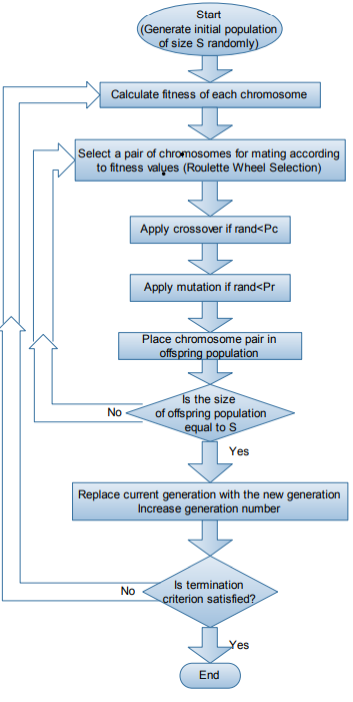
\includegraphics[width=0.4\textwidth]{diagram_1.png}
	\caption{From \cite{tartan2016flow}}
	\label{fig:Flow_1}
\end{figure}
The paper describes a 21\% improvement with their methods compared to Ghareib paper \cite{gharieb2005optimal} on the same problem. As this problem is not interlay equal to this study, comparison with this would not give a representative outcome. However, by following the approach in the paper, simulations were executed for the problem space and compare the results to results given with (theoretically) more suited genetic operations.

\newpage

\begin{figure}[ht]
	\centering
	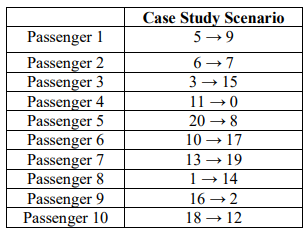
\includegraphics[width=0.4\textwidth]{tabel_1.png}
	\label{fig:Tabel_1}
	\caption{From \cite{ahmed2022investigation}}
\end{figure}

A paper\cite{ahmed2022investigation} investigates for different approaches in terms of algorithm to the problem at hand. One of its algorithm to solve the elevator dispatching problem is a genetic algorithm where the paper use Davis-order crossover, swap mutation and calculate average time for occupants  which is used as fitness function. The paper's building (problem space) and predefined settings were as following:

The results from their test show that GA where the best performing algorithm for this problem with the definitions above.

This study presents results that later compare to this study with this study's first implementation as given of the flow chart \cite{tartan2016genetic} as well as later implementation with updated genetic operations. Given the paper's result for testing different algorithms on the problem, a genetic algorithm approach seems to contribute with the best result to the elevator dispatching problem.

Another paper\cite{lim2017crossover} shortly describes different types of crossover and mutation operations. The paper describes Wright's heuristic crossover and categorized it as one of the crossover functions how offspring are “in the exploration region near the parents”\cite{lim2017crossover}. This reduces premature offspring by overcoming local minimum. Further investigation into different implementations of heuristic crossover, the concept seemed as a good crossover function for this study problem due to its simplicity and ability to be largely modified to suit the reports problem and fitness function.


